\section{RESULTATEN EN DISCUSSIE}
Het onderzoek werd gedaan met behulp van de programmeertaal Python (versie 3.12). Er werd gebruik gemaakt van de standaard library \cite{unknown-author-no-date-python}. Verder werden volgende library's nog gedownload:
\begin{itemize}
    \item numpy (versie 1.26.4)
    \item matplotlib.pyplot (versie 3.8.3)
    \item emcee (versie 3.1.4)
    \item scipy (versie 1.12.0)
\end{itemize}
\subsection{Visualisatie van het Metropolis algoritme}
In het Metropolis algoritme worden samples genomen van een gewenste kansdichtheid. Er wordt steeds begonnen vanaf een gekozen positie. In het begin kan er niet veel afgeweken worden van die positie doordat er steeds maar kleine stapjes gezet worden. De eerste data die gegenereerd wordt komt dan ook nog niet goed overeen met de gewenste kansverdeling. Daarom worden steeds de eerste gegenereerde datapunten weggegooid. \\ \\
Om dit te laten zien werd een klein programma geschreven dat probeert om een kansverdeling na te maken. Om de 90 stappen wordt de stand van zaken afgebeeld op een figuur waarop zowel de huidige kansverdeling als de gewilde kansverdeling te zien zijn. \\ \\Deze visualisatie is te zien in \cref{fig: visualisatie_metropolis}.
\begin{figure}
    \centering
    \begin{minipage}{0.49\linewidth}
        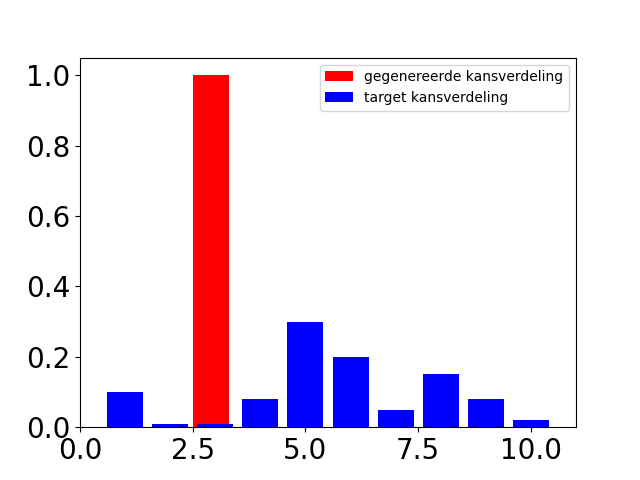
\includegraphics[width=\linewidth]{Figures/goede_visualisatie_3/visualisatie_1.png} 
        \subcaption{na stap 0}
    \end{minipage}
    \hfill
    \begin{minipage}{0.49\linewidth}
        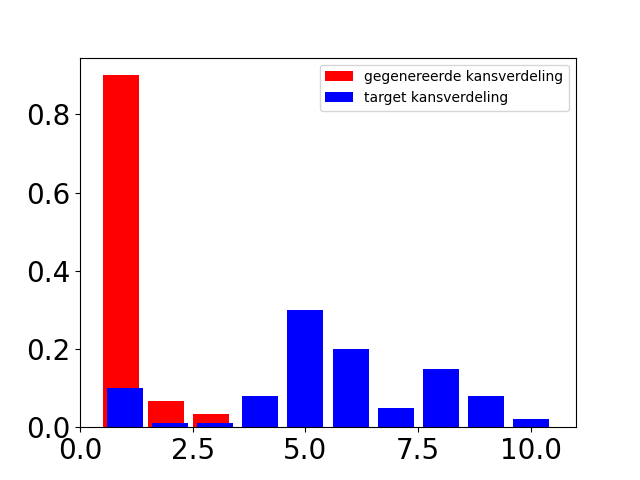
\includegraphics[width=\linewidth]{Figures/goede_visualisatie_3/visualisatie_90.png}
        \subcaption{na stap 90}
    \end{minipage}
    \begin{minipage}{0.49\linewidth}
        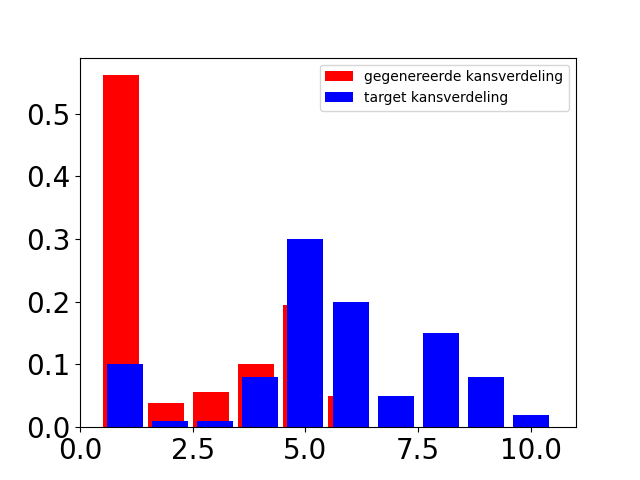
\includegraphics[width=\linewidth]{Figures/goede_visualisatie_3/visualisatie_180.png} 
        \subcaption{na stap 180}
    \end{minipage}
    \hfill
    \begin{minipage}{0.49\linewidth}
        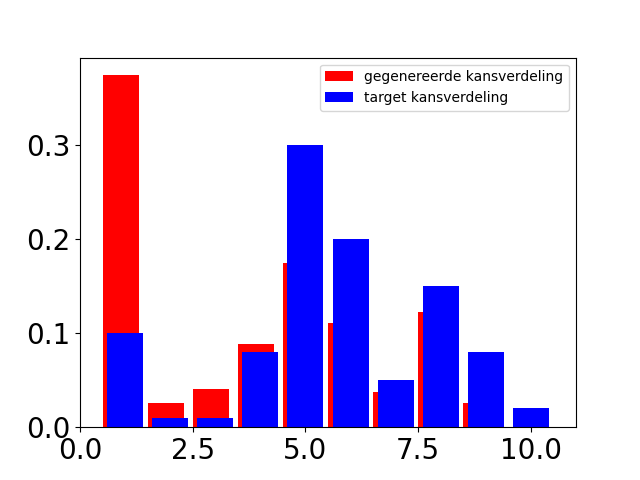
\includegraphics[width=\linewidth]{Figures/goede_visualisatie_3/visualisatie_270.png}
        \subcaption{na stap 270}
    \end{minipage}
    \begin{minipage}{0.49\linewidth}
        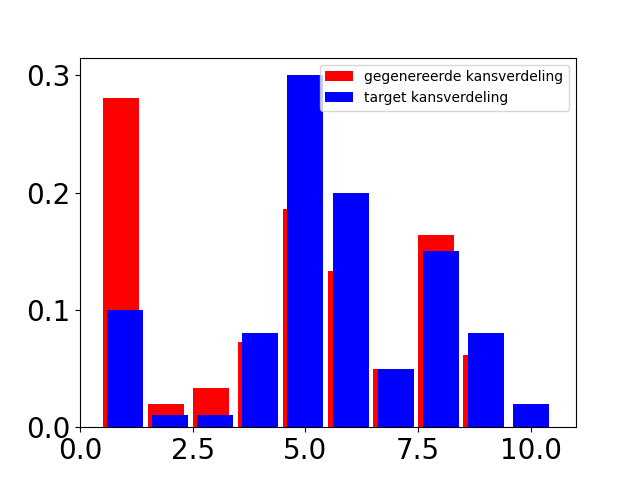
\includegraphics[width=\linewidth]{Figures/goede_visualisatie_3/visualisatie_360.png} 
        \subcaption{na stap 360}
    \end{minipage}
    \hfill
    \begin{minipage}{0.49\linewidth}
        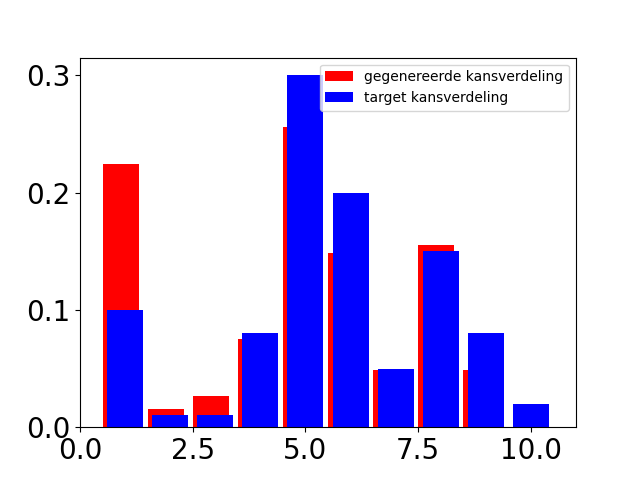
\includegraphics[width=\linewidth]{Figures/goede_visualisatie_3/visualisatie_450.png}
        \subcaption{na stap 450}
    \end{minipage}
    \begin{minipage}{0.49\linewidth}
        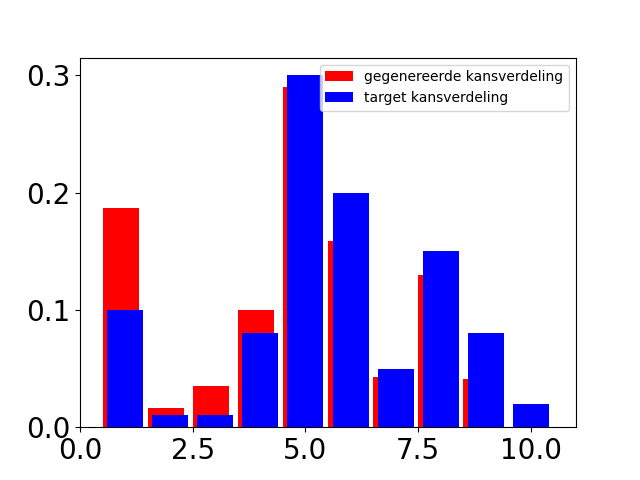
\includegraphics[width=\linewidth]{Figures/goede_visualisatie_3/visualisatie_540.png} 
        \subcaption{na stap 540}
    \end{minipage}
    \hfill
    \begin{minipage}{0.49\linewidth}
        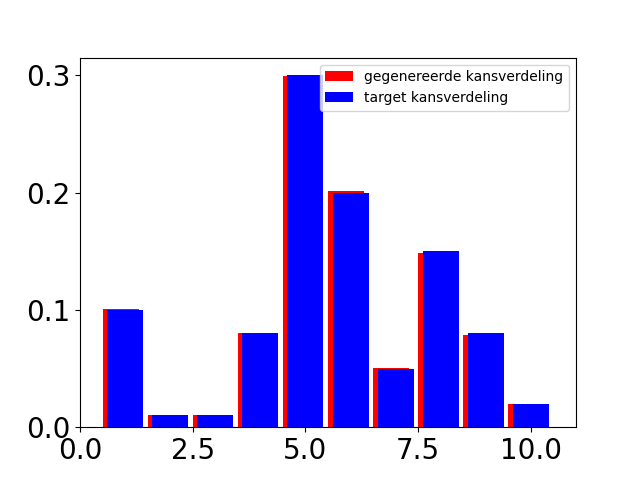
\includegraphics[width=\linewidth]{Figures/goede_visualisatie_3/visualisatie_1000000.png}
        \subcaption{na stap 100\_000}
    \end{minipage}
\caption{Visualisatie van het proces waarin toegewerkt wordt naar de gewenste kansverdeling. Op de bovenstaande figuren is de stand van zaken te zien na een vermeld aantal stappen. Het blauwe histogram is de target kansverdeling, het rode histogram is de huidige gesampelde kansverdeling.}
\label{fig: visualisatie_metropolis}
\end{figure}
Zoals te zien in de visualisatie (\cref{fig: visualisatie_metropolis}) heeft het algoritme wat tijd nodig om tot zijn target kansverdeling te komen. Na 90 stappen wordt de target kansverdeling nog niet benaderd, na 100\_000 stappen wordt bijna exact dezelfde kansverdeling als de target kansverdeling gevonden. Doordat die tijd nodig is om naar de target kansverdeling te gaan, heeft het pas zin om samples te halen uit de gewenste kansverdeling vanaf het moment dat de target benaderd wordt. Om die reden worden heel vaak de eerste samples weggegooid. Zo start de sampeling pas vanaf het moment dat de target kansverdeling bij benadering bereikt is. Het exacte punt waarop de kansverdeling goed genoeg benadert wordt, is niet gekend.
\subsection{Signaal en achtergrondruis: stelling van Bayes, het Metropolis algoritme en de emcee library}
Voor er gestart werd met het schatten van de parameters van het sterrenstelsel en het beeld dat erachter staat, werd er gestart met het afschatten van een amplitude van een signaal (A) in de aanwezigheid van achtergrondruis (B) \cite{sivia-2006}. Op de $x$-as staat de te meten variabele. De situatie is te zien in \cref{fig:AB}. 
\begin{figure}
    \centering
    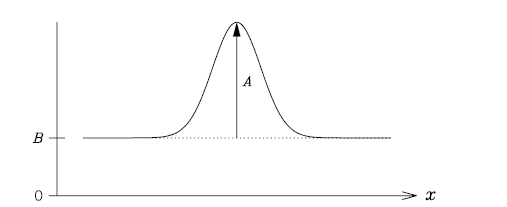
\includegraphics[width=0.95\linewidth]{Figures/Schermafbeelding 2024-05-13 144419.png}
    \caption{het meest eenvoudige geval van en signaal met amplitude A op een vlakke achtergrond van sterkte B. Foto uit \cite{sivia-2006}.}
    \label{fig:AB}
\end{figure}
Het is eenvoudig in te zien dat het aantal tellingen op een positie $x_{k}$ evenredig is met de sterkte van de achtergrond B plus het signaal A. Er wordt aangenomen dat de piek van het signaal Gaussisch is. Beschouw een piek met breedte $w$ gecentreerd rond $x_{0}$, dan is de waarde op positie $k$ gegeven door \cref{for:signaal}
\begin{equation}
D_{k}=n_{0}\left(Ae^{-\frac{(x_{k}-x_{0})^{2}}{2w^{2}}} + B\right)
\label{for:signaal}
\end{equation}
Hierin is $n_{0}$ een constante gerelateerd aan de duurtijd van de meting. \\ \\
Dit werd gedaan gebruikmakende van de stelling van Bayes. Eerst werd er gewerkt met de kansdichtheidsfunctie en later ook met het Metropolis algoritme en de emcee library. \\ \\Van de piek van het signaal en de achtergrond werd een 2D histogram gemaakt. De waarden werden ook gemarginaliseerd zodat ook het signaal en de achtergrond apart geplot konden worden. Ook werden op verschillende meetpunten $k$ het aantal tellingen bepaald. De figuren voor 1842 metingen en 25 databins, gebruikmakende van de kansdichtheid, het metropolis algoritme en de emcee library zijn te vinden in \cref{fig:AB-bay} en \cref{fig:AB-met-mc}. Merk op dat er steeds met dezelfde dataset gewerkt wordt in alle drie de voorbeelden.
\begin{figure}
    \begin{minipage}{0.95\linewidth}
        \centering
        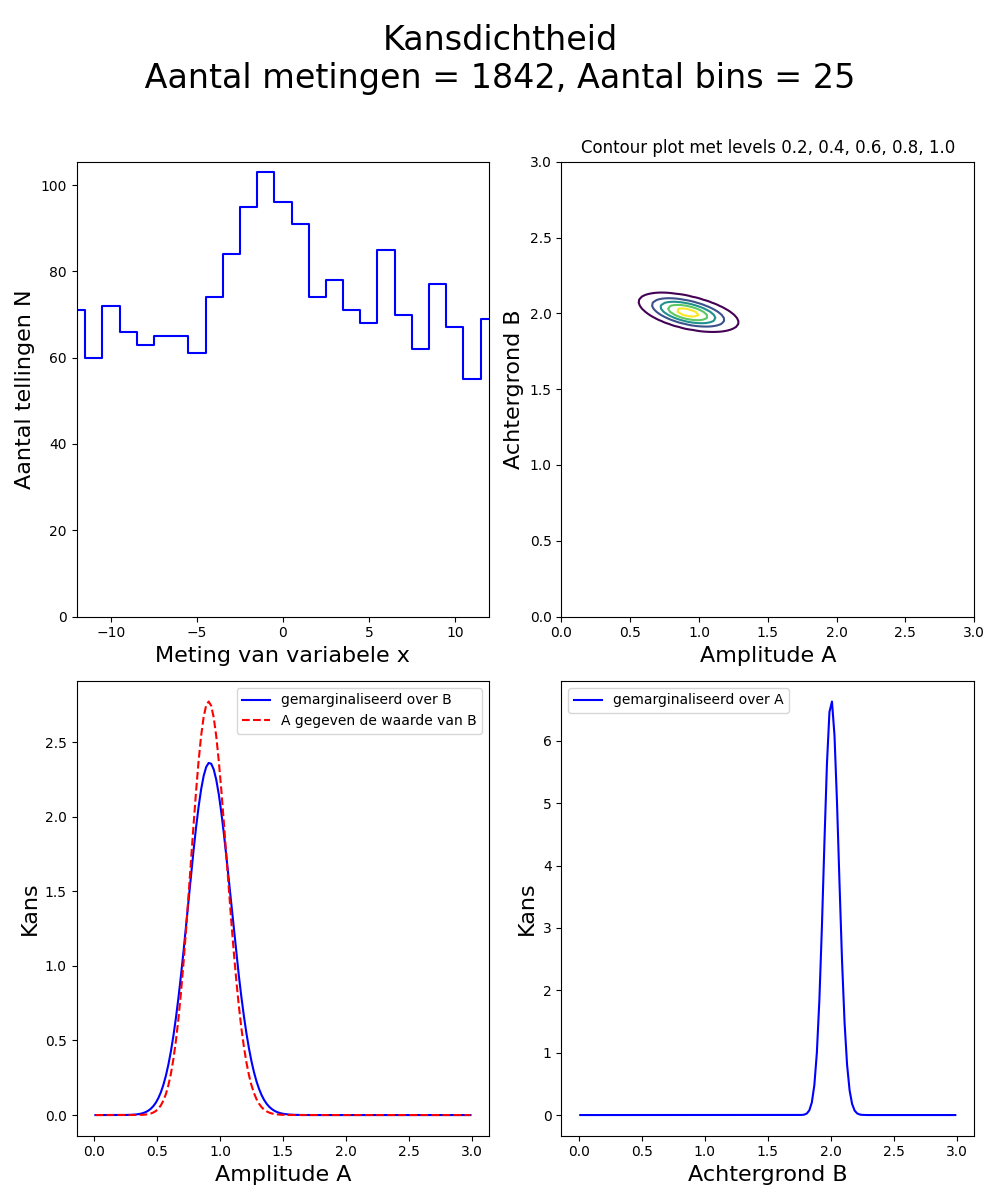
\includegraphics[width=0.95\textwidth]{Figures/figurenset1.png}
        \label{fig:AB-bayes}
    \end{minipage}
\caption{Het resultaat van het plotten van het signaal met ruis gebruikmakende van de kansdichtheid. Op de figuur linksboven staat steeds het aantal tellingen per datapunt, op de figuur rechtsboven staat het 2D histogram van het signaal met de achtergrond. Op de figuur linksonder staat de amplitude van het signaal, gemarginaliseerd over de achtergrond. Linksonder staat de achtergrond, gemarginaliseerd over het signaal.}
\label{fig:AB-bay}
\end{figure}
\begin{figure}
\begin{minipage}{0.98\linewidth}
        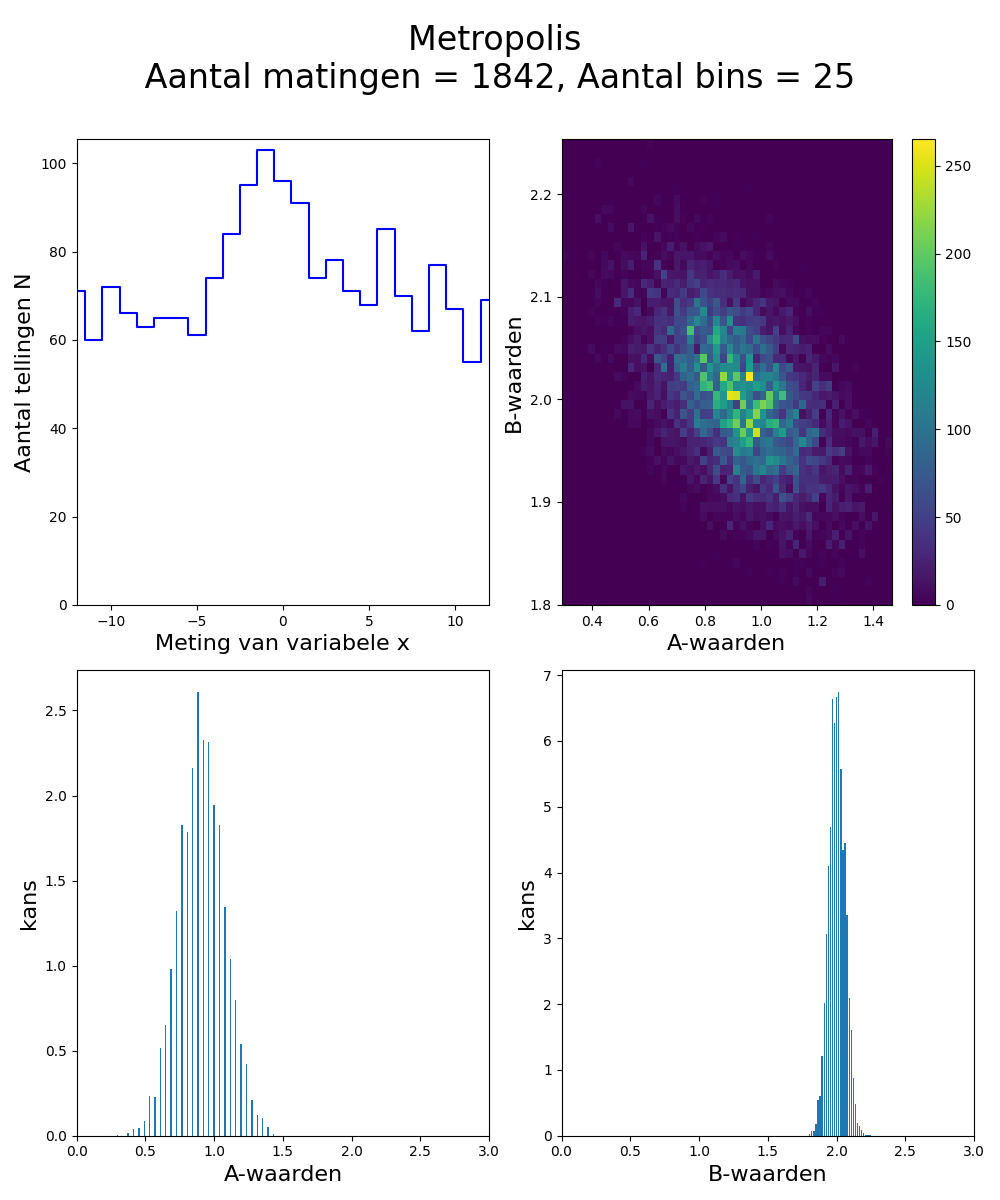
\includegraphics[width=0.95\linewidth]{Figures/signaal_AB_samples_100000.png}
        \subcaption{Figuren gegenereerd met het Metropolis algoritme.}
        \label{fig:AB-metropolis}
        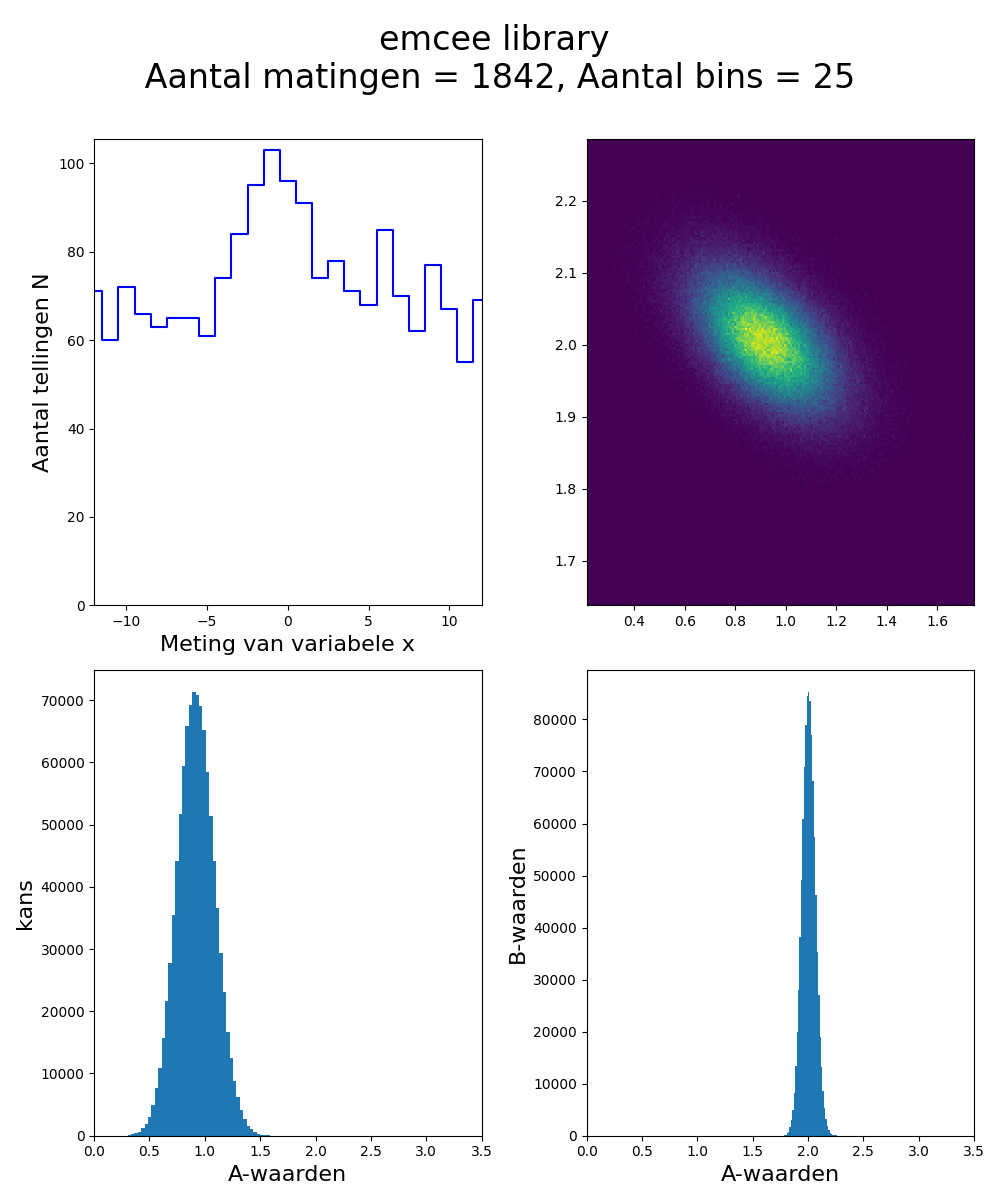
\includegraphics[width=0.95\linewidth]{Figures/emcee_hist_AB.png}
        \subcaption{Figuren met de emcee library.}
        \label{fig:AB-emcee}
    \end{minipage}
    \caption{Op de figuren staat exact hetzelfde als bij \cref{fig:AB-bay}. Hier werd er gewerkt met het Metropolis algoritme en de emcee library.  Het valt op dat de plots voor alle drie de manieren gelijkend zijn.}
    \label{fig:AB-met-mc}
\end{figure}\mbox{}\\
De figuren gegenereerd met het metropolis algoritme, met 1\_000\_000 metingen, waarvan er 60\_000 verwaarloosd zijn, zijn te vinden in \cref{fig:AB-metropolis}. \\ \\
De figuren gegenereerd met de emcee library zijn te vinden in \cref{fig:AB-emcee}. Hier werden 100 walkers gebruikt. Er werden 10\_000 datapunten gegenereerd, waarvan er 3\_000 weggegooid werden.
\\ \\
Er kan geconcludeerd worden dat de drie manieren van werken equivalente resultaten opleveren. De gevonden data is in de drie gevallen dezelfde, de pieken blijven op dezelfde plaats staan.
\subsection{Afschatten van de parameters van een sersic}
Voor het modelleren van het lichtintensiteitsprofiel van het helder sterrenstelsel wordt er gewerkt met een 2D-sersic
\cite{unknown-author-no-date-sersic}
\cite{wikipedia-contributors-2024}. Die 2D-sersic beschrijft hoe de intensiteit van een sterrenstelsel varieert met de afstand ten opzichte van het centrum. In formulevorm is dat dan gegeven door \cref{for: sersic}.
\begin{align}
    I(R)=I_{e}exp\left(b_{n}\left[\left(\frac{R}{R_{e}}\right)^{1/n}-1\right]\right)
    \label{for: sersic}
\end{align}
In \cref{for: sersic} is $I_{e}$ de amplitude, $b_{n}$ is een gammafunctie. $R_{e}$ is de effectieve straal, R is de afstand tot het middelpunt en n is de index van het profiel. Er wordt steeds gewerkt met index 1.\\ \\
Zo'n intensiteitsprofiel kan eenvoudig geplot worden met Python. Voor het plotten van een sersic moeten er zes parameters gekend zijn \cite{unknown-author-no-date-info-sersic};
\begin{enumerate}
    \item $x_{0}$: de $x$-positie van het middelpunt van het object
    \item $y_{0}$: de $y$-positie van het middelpunt van het object
    \item mate van ellipticiteit: een waarde tussen 0 en 1 waarbij 0 een cirkel is en 1 een parabool
    \item $r_{eff}$: de effectieve straal van het object, de straal waarbinnen de helft van het licht uitgestraald wordt \cite{wikipedia-contributors-2023-reff}
    \item amplitude: de helderheid van het object op een afstand $r_{eff}$ van het middelpunt
    \item $\theta$: de rotatiehoek van het object in radialen
\end{enumerate}
Stel al deze waarden zijn gekend, en zijn gelijk aan ($x_0$, $y_0$, ellips, $r_{eff}$, amplitude, $\theta$) = (100, 100, 0.3, 25, 1, $\frac{\pi}{4}$),
dan kan de 2D sersic getekend worden. Deze is te zien in \cref{fig: 2D_sersic}.
\begin{figure}
    \centering
    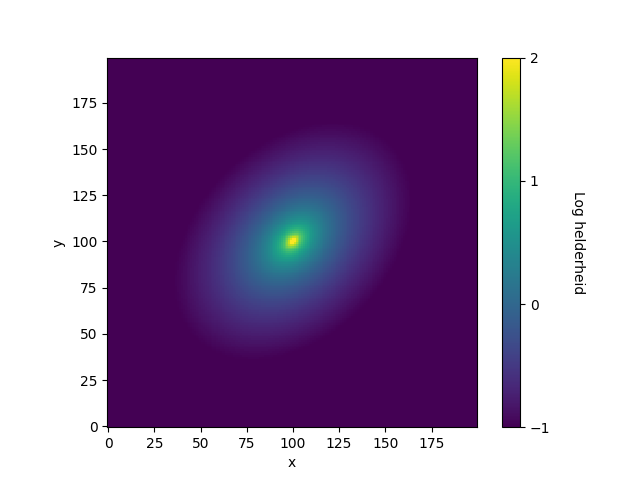
\includegraphics[width=0.95\linewidth]{Figures/figuur_2D_zonder_package_1_25_8_0.3_0.7853981633974483.png}
    \caption{Plot van een 2D sersic profiel met volgende parameters: ($x_0, y_0$, ellips, amplitude, $\theta$, $r_{eff}$) = (100,100,0.3,1,$\frac{\pi}{4}$,25).}
    \label{fig: 2D_sersic}
\end{figure}
Wat nu geprobeerd wordt is de afschatting van de zes parameters, gegeven een object. Hiervoor wordt opnieuw gebruik gemaakt van het Metropolis algoritme of van de emcee library. 
\subsubsection{De afschatting van de parameters van een sersic}
Om te beginnen wordt er gebruik gemaakt van het Metropolis algoritme. Om de complexiteit gradueel op te voeren wordt eerst enkel $x_{0}$ afgeschat, waarna ook $y_{0}$, de excentriciteit ... volgen. Wanneer niet alle parameters geschat worden, worden de resterende parameters als gekend beschouwd. Er wordt een dataset gesimuleerd op basis van de echte waarden van het object. Om de situatie meer waarheidsgetrouw te maken, wordt op de dataset poissonruis toegevoegd. Uit de posterior (die verteld hoe waarschijnlijk een combinatie van parameter is), wordt dan gesampled, in de hoop om de parameters van het object terug te vinden uit de dataset.
Er wordt gewerkt met volgende waarden voor de parameters: ($x_0$, $y_0$, ellips, $r_{eff}$, amplitude, $\theta$) = (16, 16, 0.35, 5, 50, $\frac{\pi}{4}$). \\ \\

De resultaten gebruikmakend van het Metropolis algoritme zijn te zien in \cref{appendix: opbouw}. Het eindresultaat, waarin alle zes de parameters afgeschat worden, is te zien in \cref{fig: 6 onbekenden}. Voor de afschatting van die zes parameters werden 9\_500\_000 samples gegenereerd waarvan er 1\_500\_000 weggegooid werden.
\begin{figure}
    \centering
    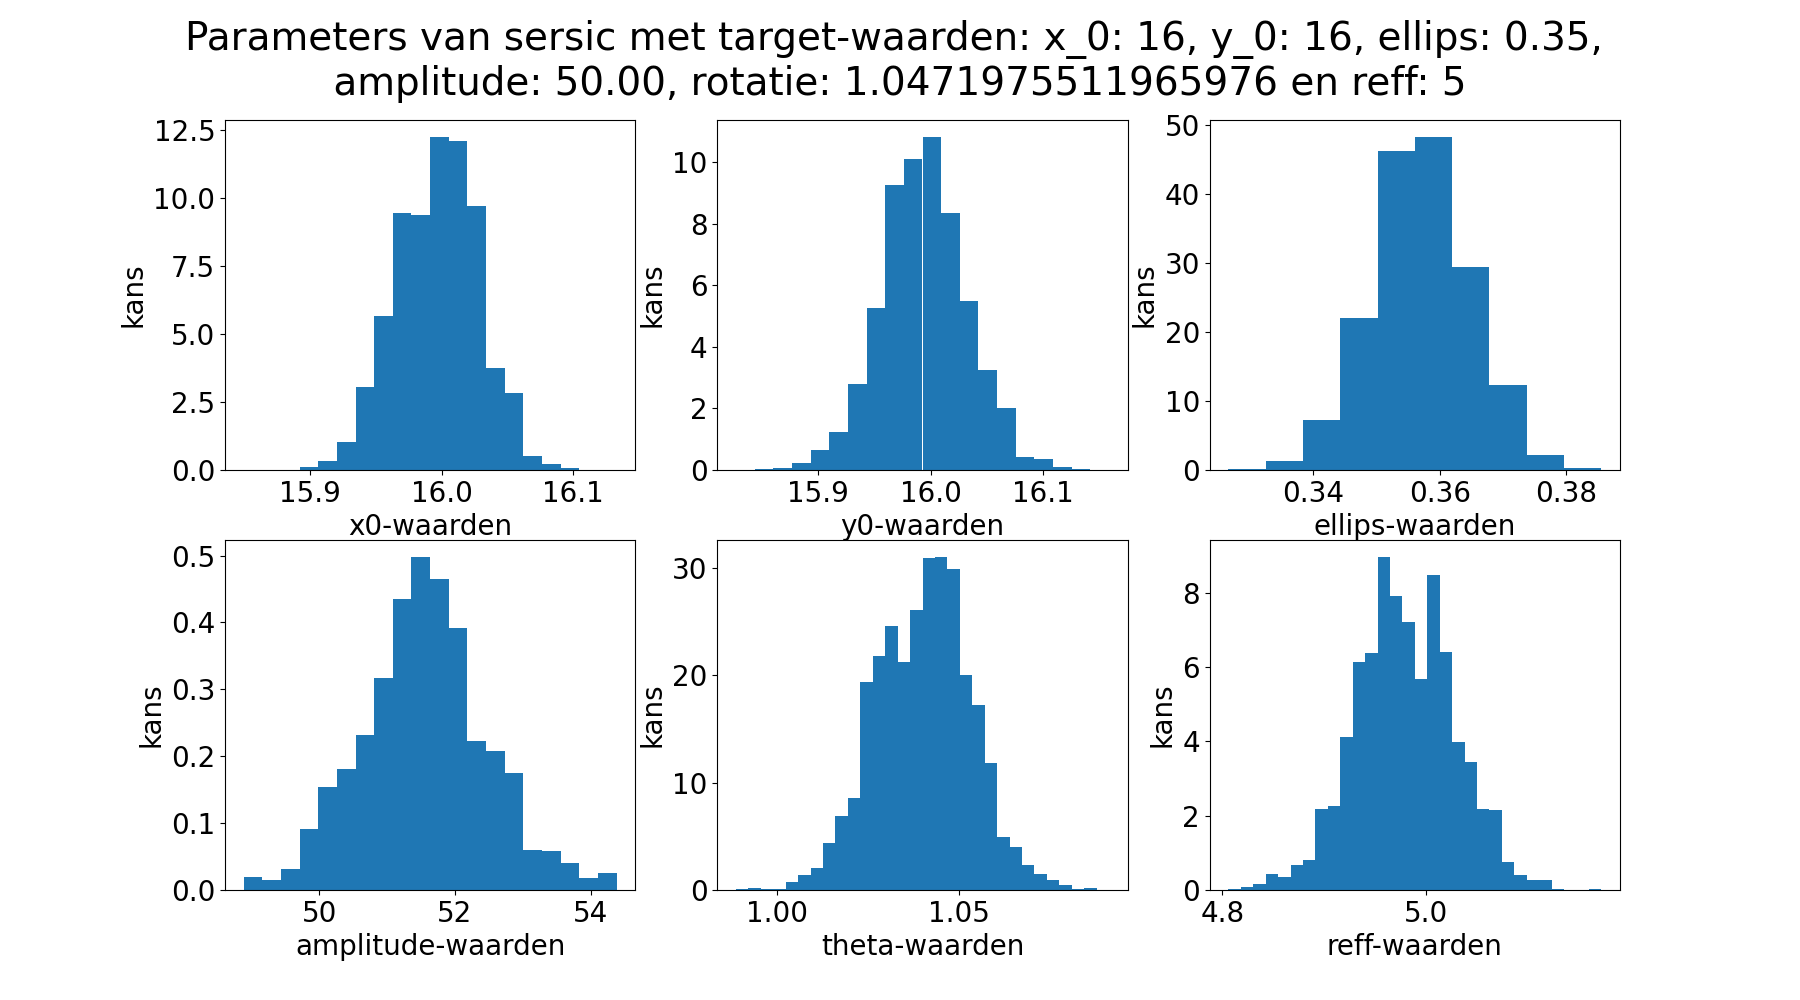
\includegraphics[width=0.95\linewidth]{Figures/sersic_parameters_metropolis_9500000_1500000_50_reff.png}
    \caption{Het resultaat van de afschatting van zes verschillende parameters van de sersic met waarden ($x_0,\ y_0$, ellips, amplitude, $\theta$, $r_eff$) = (16, 16, 0.35, 50, $\frac{\pi}{3}$,  5).}
    \label{fig: 6 onbekenden}
\end{figure}
Zoals te zien in \cref{fig: 6 onbekenden} komen de pieken van afgeschatte parameters goed overeen met de effectieve waarden die gebruikt zijn om de dataset te generen. \\ \\De afgeschatte parameters kunnen ook getoetst worden aan de bijhorende figuur van de sersic (opgebouwd op basis van de dataset die gemodelleerd is om de parameters af te schatten). Die figuur is te zien in \cref{fig: af te schatten sersic}. Op de figuur is inderdaad te zien dat de sersic ongeveer $45^{\circ}$ geroteerd is. Ook de $x_0$ en $y_0$ posities en de excentriciteit zijn te zien en komen inderdaad overeen met de waarden die afgeschat werden. 
\begin{figure}
    \centering
    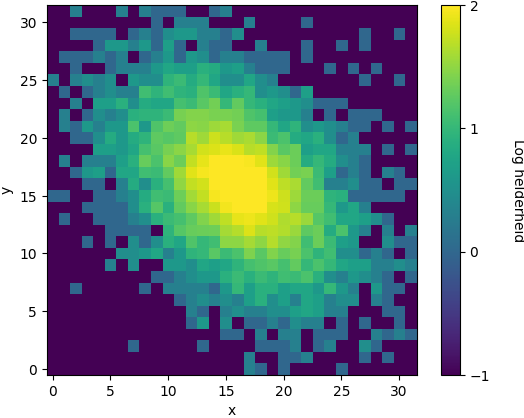
\includegraphics[width=0.95\linewidth]{Figures/sersic.png}
    \caption{Een 2D sersic gegenereerd volgens de dataset die gebruikt werd om de waarden van de sersic te zien in \cref{fig: 6 onbekenden} af te schatten.}
    \label{fig: af te schatten sersic}
\end{figure}\mbox{}\\ \\
Hetzelfde kan nu gedaan worden met behulp van de emcee library. Hier worden alle zes de parameters meteen tegelijk afgeschat. Het resultaat van de afschatting met 100 walkers, 12000 stappen, waarvan er 2300 weggegooid zijn, is te vinden in \cref{fig: emcee}.
\begin{figure}
    \centering
    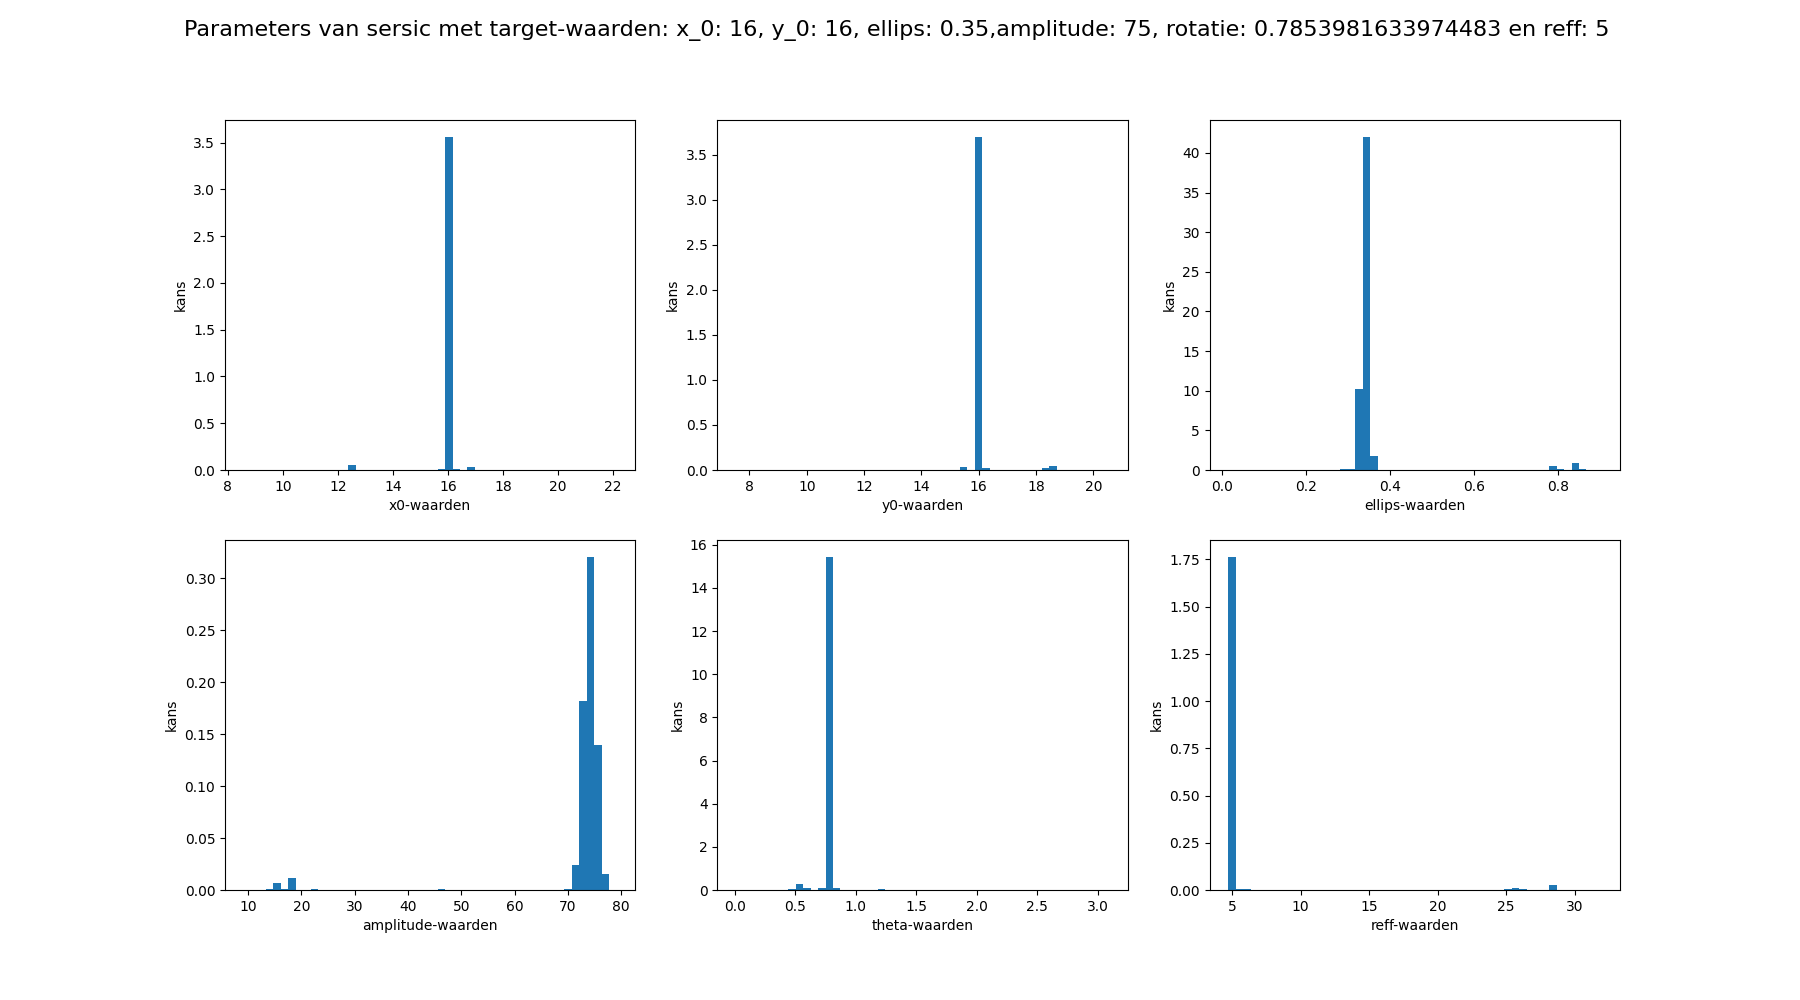
\includegraphics[width=0.95\linewidth]{Figures/emcee_hist_12000_2300.png}
    \caption{Het resultaat van het afschatten van de zes parameters van de sersic, gebruikmakend van de emcee library. De targetwaarden van deze sersic waren ($x_0,\ y_0$, ellips, amplitude, $\theta$, reff) = (16, 16, 0.35, 75, $\frac{\pi}{4}$,  5)}
    \label{fig: emcee}
\end{figure}\mbox{}\\
Opnieuw kan er een goede afschatting van de parameters van de sersic gemaakt worden. Werken met de emcee library blijft wel eenvoudiger, doordat er geen kennis van het systeem vereist is.

\subsection{Het afschatten van parameters van twee 2D sersic systemen}
Nu de parameters van één object afgeschat kunnen worden is het doel om ook de parameters van twee (of zelfs meerdere) objecten af te kunnen schatten. De werkwijze is volledig analoog aan het geval met slechts één object. Er wordt opnieuw gebruik gemaakt van zowel het Metropolis algoritme als de emcee library. \\ \\
Soms kan een object dat achter een ander object staat niet waargenomen worden. Dat wordt weergegeven in \cref{fig:2_sersic}. Daar staat op de eerste foto een eerste sersic, op de tweede foto staat een tweede sersic en op de derde foto zijn de beelden samengevoegd tot één afbeelding. \\ \\
Doordat een sersic soms verdwijnt achter een andere sersic is het nodig om de parameters van meerder objecten goed te kunnen schatten. Dit is nodig om verder te kunnen gaan in de bachelorproef. Er gaat later nog geprobeerd worden om de achtergrond waarop het sersicsysteem staat af te schatten, en dan is het belangrijk dat ook systemen met meerdere sersics afgeschat kunnen worden. 
\begin{figure}
    \centering
    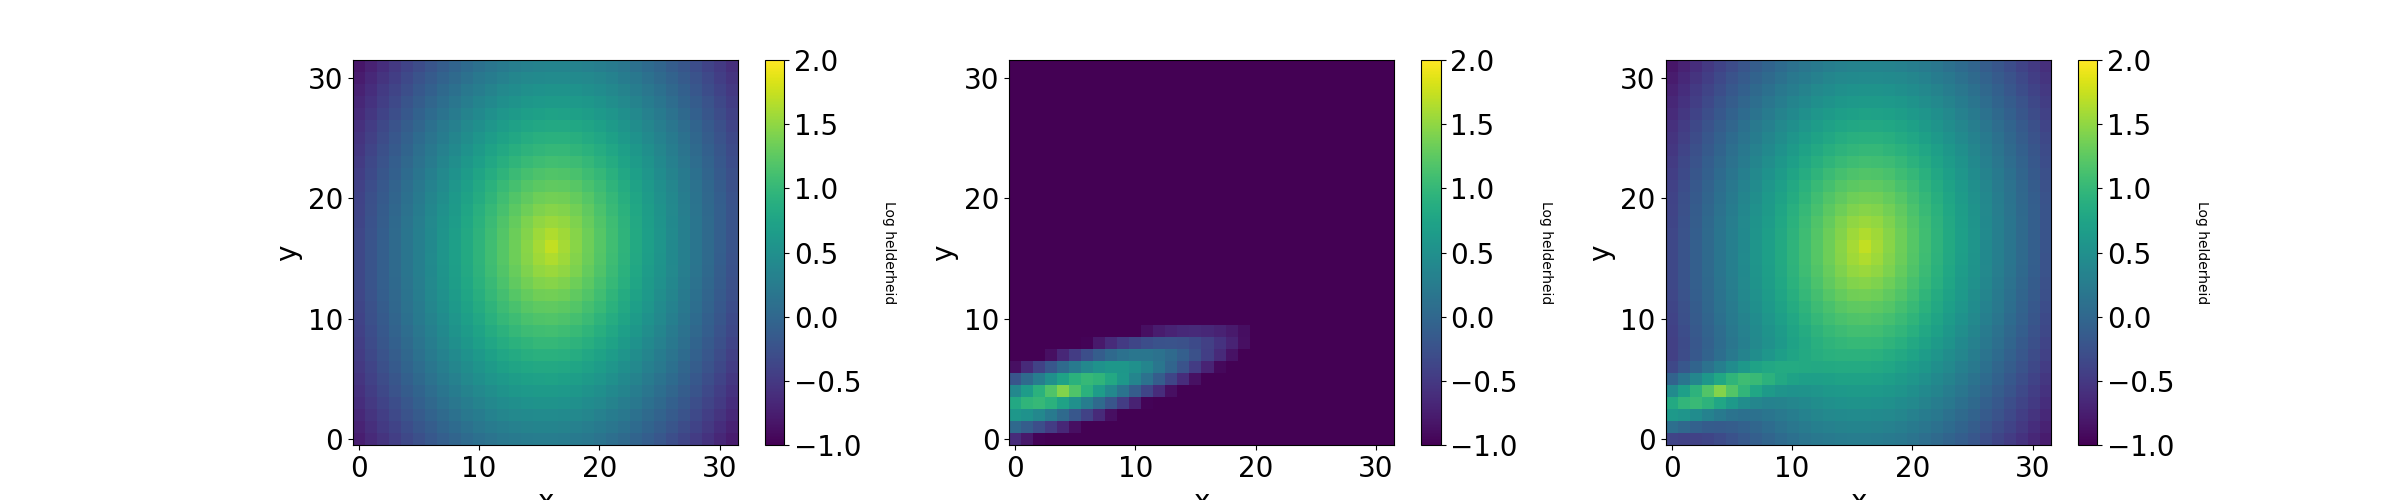
\includegraphics[width=0.99\linewidth]{Figures/figuur_2D_zonder_package_10_8_1_0.3_1.5.png}
    \caption{Op de meest linkse figuur staat een heldere sersic, op de middelste figuur staat een tweede, over het algemeen minder heldere sersic. Op de meest rechtse figuur is het resultaat van de optelling van de twee sersics te zien.}
    \label{fig:2_sersic}
\end{figure}\mbox{}\\
Er werd een eerste poging gedaan tot het afschatten van de parameters van de twee sersic profielen. De resultaten ervan zijn te zien in \cref{fig:sersic 1} en \cref{fig:sersic 2} voor respectievelijk de eerste sersic en de tweede. Wat opvalt is dat er op beide figuren twee pieken staan. Dat is logisch, doordat er ontaarding is. Het algoritme kan niet bepalen welke sersic nummer 1 is, en welke sersic nummer 2 is. De afgeschatte waarden komen overeen met wat er verwacht wordt, maar het is nu nog zaak om de juiste parameters te koppelen aan de juiste sersic.
\\ \\
In het proces van het genereren van de samples wordt er steeds een voorstel gedaan, een kans bepaald, en dan wordt een staat geaccepteerd of verworpen. Er wordt vanaf nu bijgehouden welke combinatie van parameters de hoogste kans had (hoewel het eigenlijk strikt genomen over kansdichtheden gaat). Dan is nog niet geweten welke set van parameters sersic 1 beschrijft, en welke set van parameters sersic 2 beschrijft, maar dat hoeft geen probleem te zijn. De juiste combinaties van de parameters is dan wel gekend. Het resultaat is te zien in \cref{fig: 2 sersic niet ontaard}.
\begin{figure}
    \begin{minipage}{0.98\linewidth}
        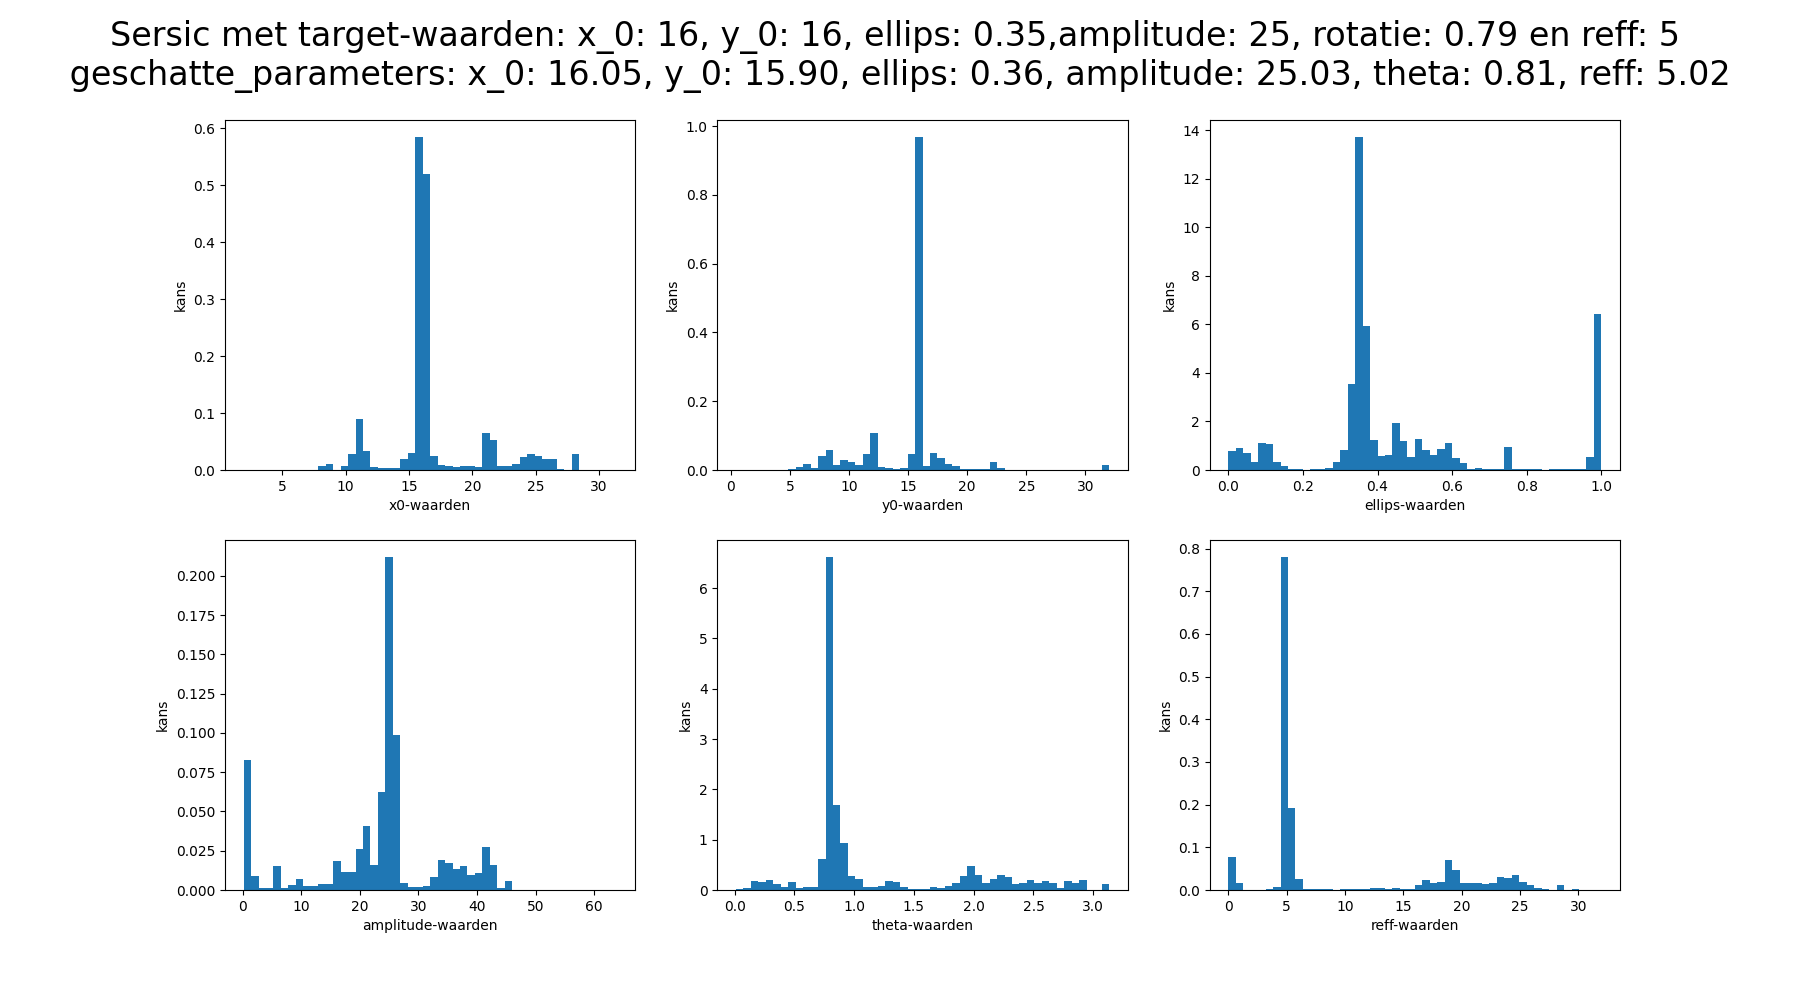
\includegraphics[width=0.95\linewidth]{Figures/1_emcee_hist_5000_750.png}   
        \subcaption{De parameters van de eerste van twee sersics}
        \label{fig:sersic 1}
        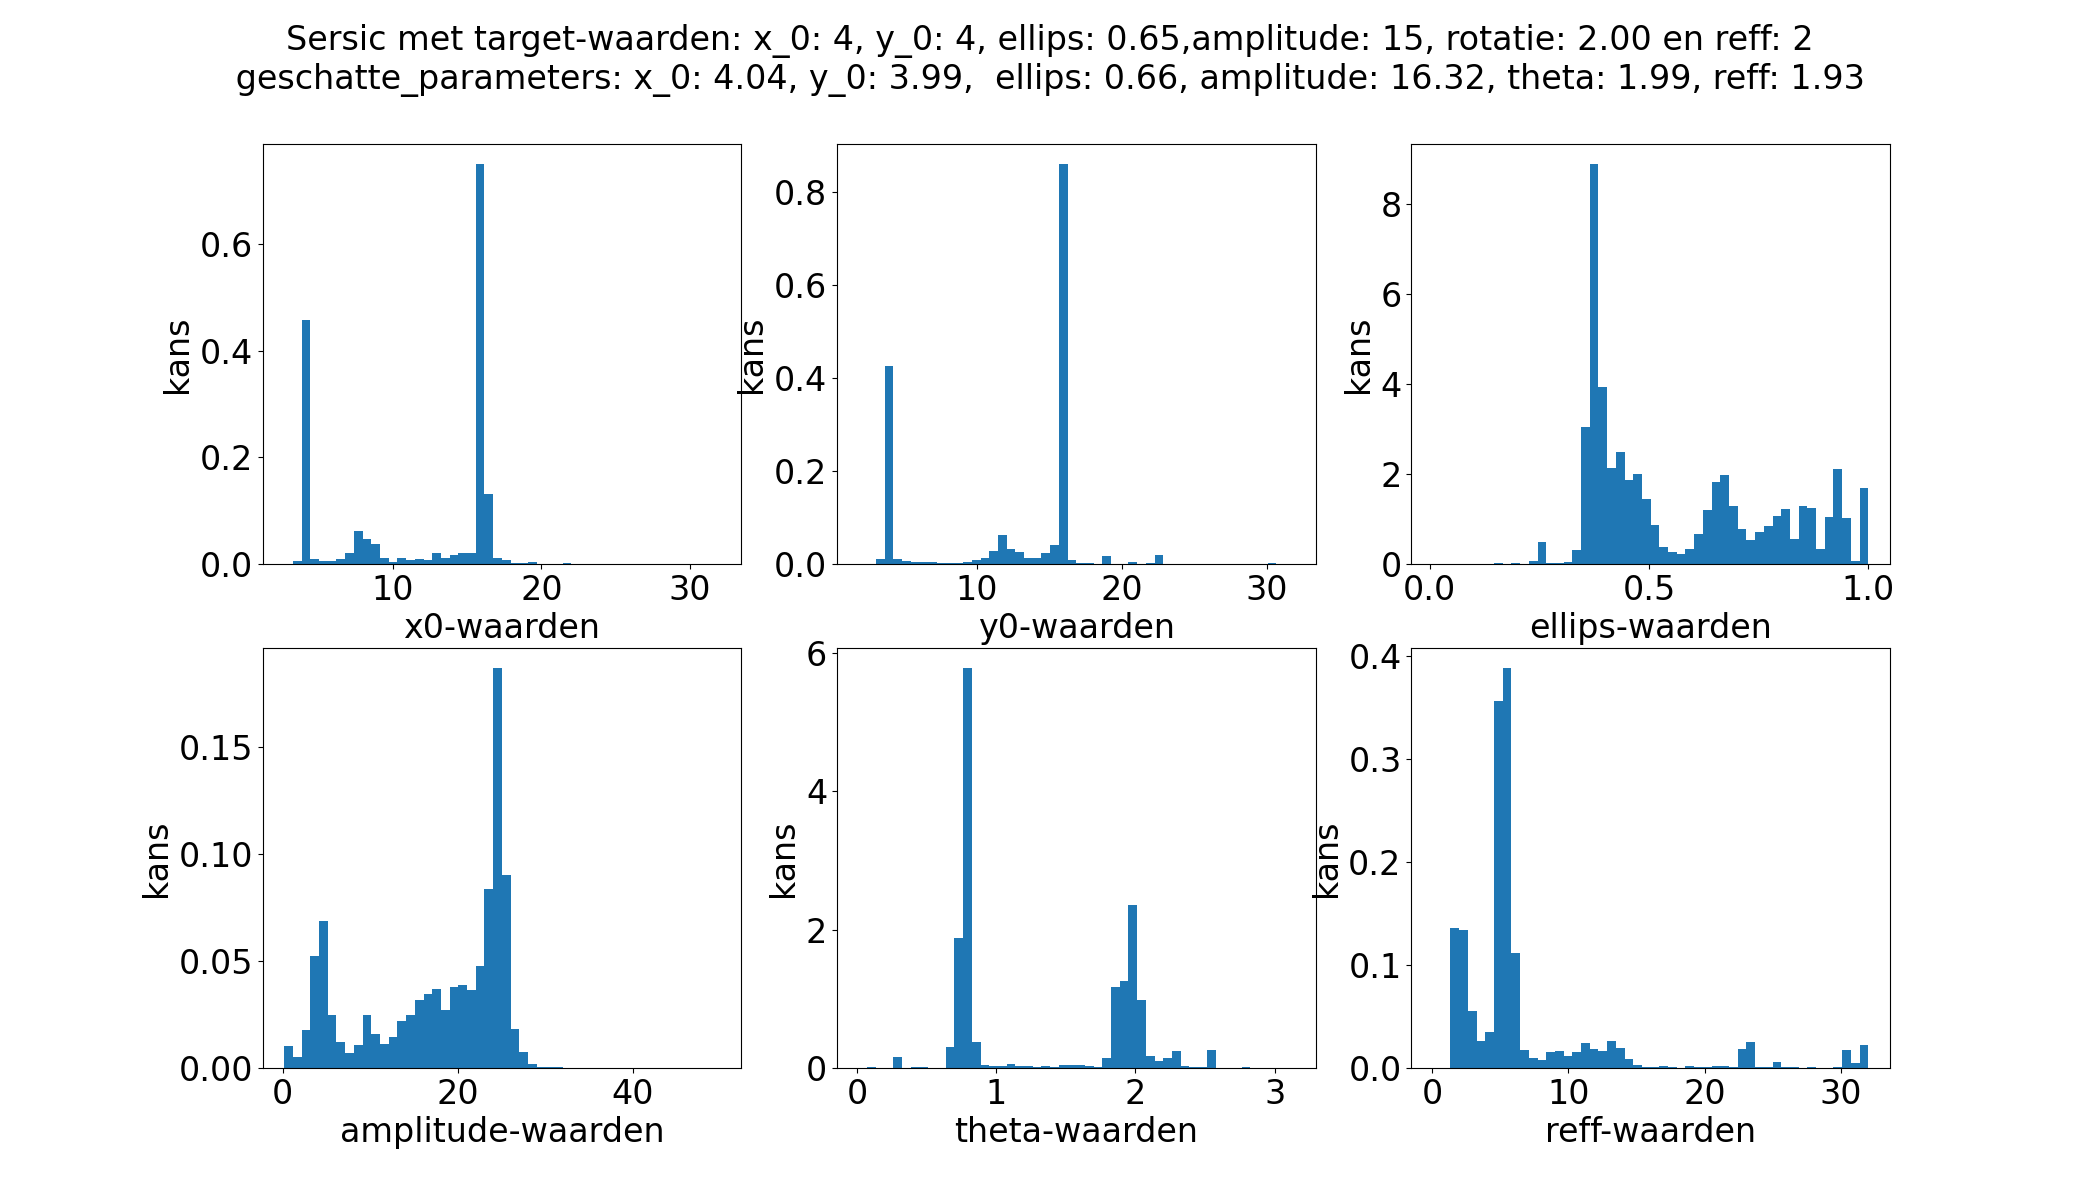
\includegraphics[width=0.95\linewidth]{Figures/2_emcee_hist_5000_750.png}
        \subcaption{De parameters van de tweede sersic}
        \label{fig:sersic 2}
        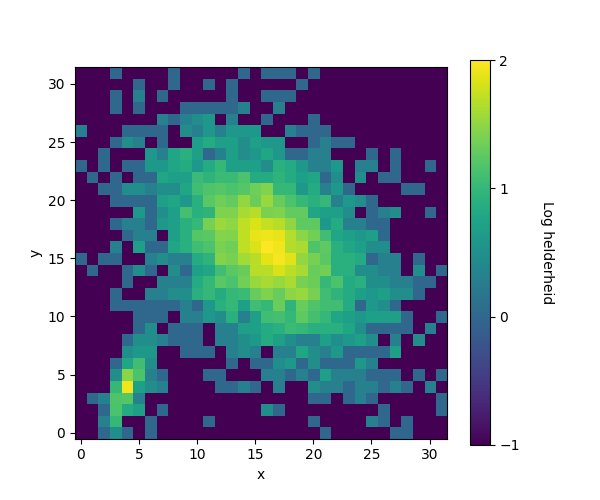
\includegraphics[width=0.95\linewidth]
        {Figures/figuur_2D_zonder_package_5000.png}
        \subcaption{Een plot van het sersicsysteem volgens de gegenereerde data.}
    \end{minipage}
    \caption{De afschatting van de parameters in het geval van twee sersic (waarbij de ene sersic naast de andere staat) in dezelfde figuur. Naast de verwachte parameters worden ook steeds de geschatte parameters weergegeven. Ook de plot van de af te schatten sersic wordt weergegeven. Op de grafieken is nog steeds ontaarding te zien, maar het koppelen van de juiste parameters lukt door gebruik te maken van onze methode van de grootste kans}
    \label{fig: 2 sersic niet ontaard}
\end{figure}
De parameters van beide sersics kunnen goed afgeschat worden. Op deze manier kan het totale sersicstelsel goed afgeschat worden. In de laatste stap van deze bachelorproef wordt er geprobeerd om de parameters van een sersic af te schatten zodat de achtergrond waarop deze sersic staan gevonden kan worden. Het is dan ook belangrijk dat eender welk sersicsysteem (ook een systeem met meerdere sersics) goed afgeschat kan worden.

\subsection{De afschatting van parameters van een 2D sersic systeem met een werkelijke achtergrond}
In de voorgaande bepaling van de parameters van het sersic profiel werd aan de dataset van de werkelijke waarden wat ruis toegevoegd. Nu wordt overgegaan op een meer werkelijke toestand door de sersic met het poissonruis te plaatsen op een achtergrond die gemodelleerd is door NASA. \\ \\
De achtergrond die gebruikt wordt is te zien in \cref{fig:NASA}. Dit is een zeer grote foto, voor de achtergrond in het programma werd een deeltje van 64x64 pixels genomen uit deze afbeelding. Zo'n figuur is te zien in \cref{fig:achtergrond nasa}.
Hierop werd dan een sersic geplaatst om zo tot een nieuw geheel te komen. Zo'n sersic op de werkelijke achtergrond is te zien in \cref{fig:achtergrond+sersic}. Dit zal uiteindelijk ook de dataset worden.
\begin{figure}
    \begin{minipage}{0.98\linewidth}
        \centering
       \includegraphics[width=0.55\linewidth]{Figures/achtergrond_groot.jpg}
        \subcaption{Een achtergrondbeeld gemodelleerd door NASA. Foto van \cite{nasa-2023}}
        \label{fig:NASA} 
        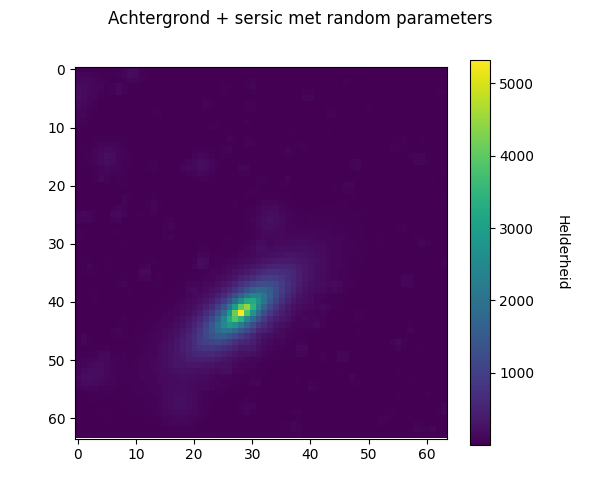
\includegraphics[width=0.85\linewidth]{Figures/sersic+achtergrond_656679_clip2.png}
        \caption{Een 2D sersic profiel op een werkelijke achtergrond.}
        \label{fig:achtergrond+sersic}
    \end{minipage}
    \caption{De opbouw van het genereren van een sersic op een werkelijke achtergrond. Eerst wordt een deeltje geknipt uit de werkelijke achtergrond (zie \cref{fig:achtergrond nasa}), er wordt een sersic gegeneerd met willekeurige parameters. De sersic wordt opgeteld bij de achtergrond en geeft zo een ruizig geheel dat de werkelijkheid weerspiegeld.}
\end{figure}
\\
Het uiteindelijke doel is nu om de waarden van de sersic af te schatten om zo enkel de achtergrond te bekomen. De afschatting van de parameters van deze sersic wordt gedaan door gebruik te maken van de emcee library.
\\ \\

Vanuit het geheel (een sersic met poissonruis geplaatst op een achtergrond) worden nu de parameters van de sersic afgeschat. Als de parameters geschat zijn wordt een afgeschatte sersic getekend (op basis van de geschatte parameters). Om dan de achtergrond te vinden wordt de geschatte sersic afgetrokken van het geheel. Zo blijft enkel de achtergrond over. De achtergrond geknipt uit het beeld van NASA is te zien in \cref{fig:achtergrond nasa}, het totaal is te zien in \cref{fig:achtergrond+sersic} en de afgeschatte achtergrond is te zien in \cref{fig:geschatte achtergrond}.
\\ \\
\begin{figure}
    \begin{minipage}{0.98\linewidth}
        \centering
        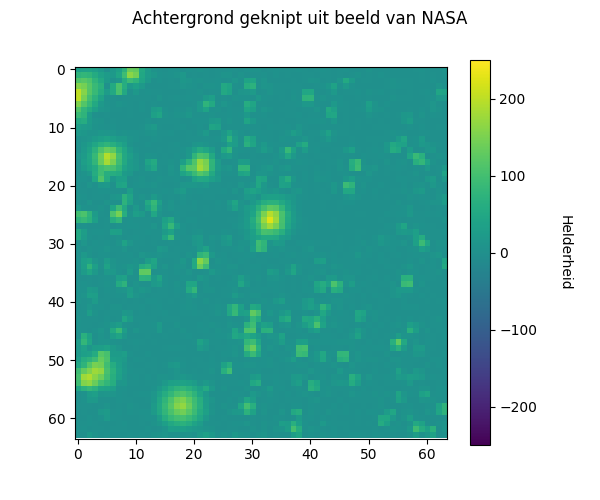
\includegraphics[width=0.95\linewidth]{Figures/sersic_achtergrond_656679_clip2.png}
        \subcaption{De achtergrond geknipt uit de gemodelleerde achtergrond van NASA}
        \label{fig:achtergrond nasa}
        \centering
        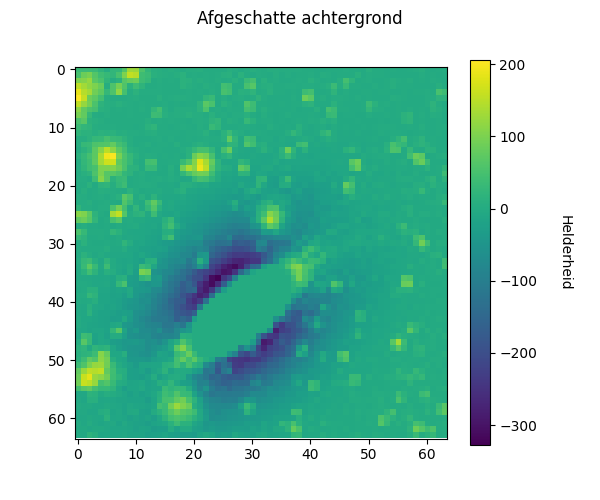
\includegraphics[width=0.95\linewidth]{Figures/afgeschatte_achtergrond_656679.png}
        \subcaption{De afgeschatte achtergrond, waarin de zes parameters van de sersic afgeschat werden.}
        \label{fig:geschatte achtergrond}
    \end{minipage}
    \caption{De vergelijking tussen de oorspronkelijke achtergrond (\cref{fig:achtergrond nasa}) de afgeschatte achtergrond (\cref{fig:geschatte achtergrond}). De sersic geplaatst op de achtergrond is te zien in \cref{fig:achtergrond+sersic}. Over het algemeen komen de figuren goed overeen, maar op de afgeschatte achtergrond is wel duidelijk te zien dat sersic niet volledig correct afgeschat is.}
\end{figure}

Op de figuren is te zien dat de afgeschatte achtergrond wel goed overeenkomt met de werkelijke achtergrond. Wat wel opvalt is dat de parameters van de sersic niet zo goed afgeschat zijn. Daardoor blijft een deel van de sersic zichtbaar en zijn we nog niet in staat om de objecten achter de sersic te zien. \\ \\
Wat verder ook opvalt is dat er sommige plaatsen teveel afgetrokken wordt van de figuur, op andere plaatsen wordt er te weinig afgetrokken. Er werd geprobeerd om ervoor te zorgen dat er nooit te veel afgetrokken zou kunnen worden, waardoor er geen negatieve waarden bekomen konden worden. Dit werkte echter niet, er werd geen enkele combinatie van waarden meer gevonden. \\ \\
In de toekomst zou het afschatten van de achtergrond ook met AI kunnen gebeuren. Er is al een dataset die bestaat uit 100 sets van de sersic + achtergrond enerzijds, en de achtergrond anderzijds. Met deze dataset zou een AI getraind kunnen worden.










